\section{Pojektstruktur}
Wir stellen im Folgenden die Strukturierung des Projektes sowie das Build-System vor.
Außerdem führen wir kurz in den Inhalt einzelner Verzeichnisse ein.\par

Die oberste Ebene der Verzeichnisstruktur von helios bietet Zugriff auf Tests, ausführbare Beispielprogramme, Benchmarks sowie Dokumentation und Quelldateien.
Die gewählte Struktur lehnt sich dabei an die durch das \textit{Pitchfork}-Projekt definierten Konventionen für C++-Projekte an~\cite[]{Pitchfork}.
Die Verzeichnisnamen geben dabei Aufschluss über den durch sie verwalteten Inhalt und ist wie in Abbildung~\ref{fig:verzeichnisstruktur} angegeben.\par

\begin{figure}[htbp]
    \setlength{\DTbaselineskip}{18pt}
    \dirtree{%
        .1 ./.
        .2 benchmarks/.
        .2 docs/.
        .2 examples/.
        .2 include/.
        .2 src/.
        .2 tests/.
    }
    \caption{Projektverzeichnis von helios (Ausschnitt).}
    \label{fig:verzeichnisstruktur}
\end{figure}

Das Projekt besitzt verschiedene Build-Schritte, um sowohl die Sourcen zu kompilieren, als auch die Tests und die Beispielprogramme zu erzeugen.
Zur Automatisierung nutzen wir \texttt{CMake}~\cite[]{CMake}, womit wir gleichzeitig ein einfaches Dependency-Management realisieren.
Die für die Entwicklung benötigten \textit{Third-Party Libraries} (TPL) (u.a. \texttt{gflw}~\cite[]{glfwHomepage} und \texttt{glad}~\cite[]{gladgithub}) können somit direkt aus externen Quellen geladen, statisch kompiliert und eingebunden werden (siehe Listing~\ref{lst:cmake}).\par

Damit automatisieren wir die Vorkonfiguration des Projektes und vermeiden manuelles (und oft fehleranfälliges~\cite[]{FG22}) Einbinden der benötigten TPLs.

\vspace{4mm}
\begin{lstlisting}[style=c++style, caption={Ausschnitt aus der CMakeLists.txt von helios: Dieser Abschnitt deklariert und bezieht GLFW v3.4 und GLAD v2.0.8 per FetchContent von den jeweiligen Github-Repositories (URLs der Übersicht halber ausgelassen). Im Anschluss wird ein GLAD-Loader für OpenGL 4.6 als statische Bibliothek erzeugt.}, label=lst:cmake]
    ...
    FetchContent_Declare(glfw
        GIT_REPOSITORY [url]
        GIT_TAG        3.4
    )

    FetchContent_Declare(glad
        GIT_REPOSITORY [url]
        GIT_TAG        v2.0.8
        SOURCE_SUBDIR  cmake
    )
    FetchContent_MakeAvailable(glfw glad)

    #GLAD v2: Core GL 4.6
    glad_add_library(
        glad_gl_core_46
        STATIC REPRODUCIBLE LOADER API
        gl:core=4.6
    )
    ...
\end{lstlisting}
\vspace{4mm}

\subsection{Verzeichnisinhalte}

Im Folgenden stellen wir die Hauptverzeichnisse in alphabetischer Reihenfolge vor und gehen dabei kurz auf deren Inhalte ein.


\subsection*{\texttt{benchmarks}}
Zum Benchmarking einzelner Funktionen nutzt helios \textit{Google Benchmark}~\cite[]{googlebenchmarkgithub}.
Es existieren derzeit Benchmarks für mathematische Typen und Funktionen.
Wir nutzen diese für einen Vergleich mit der Implementierung in \texttt{glm}~\cite[]{glmGithub}, die wir als Referenz betrachten.
Hierdurch sollen frühzeitig Flaschenhälse in der \textit{Game Loop} - bspw. durch Operationen auf affinen Transformationsmatrizen - erkannt werden.
Weitere Benchmarks, die das Verhalten ausgewählter Funktionen der \textit{Rendering Pipeline} bzw. der \textit{Application Stage}~\cite[687]{Gre19} messen (bspw. beim Culling), sollen folgen.




\setlength{\tabcolsep}{8pt}
\begin{table}[t]
    \centering
    {\renewcommand{\arraystretch}{1.2}%
    \begin{tabular}{lrrr}
        \hline
        \textbf{Benchmark} & \textbf{Time} & \textbf{CPU} & \textbf{Iterations} \\
        \hline
        BM\_mat4Constructor/real\_time         & 5.81 ns  & 5.85 ns  & 106{,}874{,}145 \\
        BM\_glm\_mat4Constructor/real\_time    & 13.0 ns  & 13.1 ns  & 53{,}781{,}740 \\
        BM\_mat4Multiply/real\_time            & 175 ns   & 168 ns   & 3{,}896{,}895 \\
        BM\_glm\_mat4Multiply/real\_time       & 430 ns   & 434 ns   & 1{,}655{,}019 \\
        \hline\\
    \end{tabular}}
    \caption{Beispielausgabe von Benchmark-Ergebnissen, hier anhand der eigenen \texttt{mat4}
    \label{tab:mat4-benchmark}-Implementierung im Vergleich zu \texttt{glm::mat4} unter (nicht repräsentativen) Laborbedingungen.}
\end{table}


Eine Evaluation von Benchmarking-Frameworks fand nicht statt, die Auswahl richtete sich nach Popularität und Empfehlungen.

\subsection*{\texttt{/docs}}
Das Verzeichnis enthält neben formaler Dokumentation\footnote{wie den \LaTeX-Quelltext des vorliegenden Dokuments} die auf den Quelldateien beruhende und von \texttt{doxygen}~\cite[]{Doxygen} erzeugte API-Dokumentation.
\texttt{doxygen} hat den Vorteil, dass es eine Überführung in verschiedene Formate erlaubt.
Hierdurch können wir die Dokumentation im html- bzw. xml-Format exportieren und durch einen gesonderten Build-Schritt in die helios-Projektwebseite~\cite[]{helios} einbinden.\par

Eine formale Evaluation von Software-Dokumentationstools hat nicht stattgefunden.
Die Auswahl basierte auf Grundlage der leichten Integration von \texttt{doxygen} und seiner Bekanntheit.
Zudem sehen wir die umfangreiche Auswahl an verschiedenen Ausgabeformate (u.a. PDF, Markdown) zur Unterstützung der Projektdokumentation als Vorteil.


\subsection*{/tests}
Für das Unit Testing verwendet helios \textit{Google Test}~\cite[]{googletestgithub}.
Wir streben eine kurzfristige Erhöhung der Entwicklungsgeschwindigkeit unter Annahme eventueller Projektinstabilität an, weshalb wir zu Projektbeginn keine hohe Testabdeckung eingeplant haben.
Aus diesem Grund liegt der Schwerpunkt der Tests derzeit auf den mathematischen Funktionen, um beispielsweise Transformationen innerhalb des Szenengraphen zu validieren. helios nutzt \texttt{glm} als Testorakel~\cite[917 ff.]{Bin99}, um Ergebnisse abzugleichen\footnote{
    Alternativ lässt sich \texttt{glm} als \textit{baseline} auffassen, gegen die die Funktionen in helios (als \textit{delta version}) in Regressions-Tests verglichen werden. Uns ist bewusst, das sich eventuelle Fehler in \texttt{glm} direkt auf die Implementierung in helios auswirken. Wir bewerten dieses Risiko aufgrund der Projektreife von \textit{glm} als äußerst gering.
}.

Wie bei dem Benchmarking fand keine Evaluation unterschiedlicher Unit-Test-Frameworks statt.
Wir haben uns an Popularität und Empfehlungen orientiert.

\subsection*{\texttt{/examples}}
Das Verzeichnis enthält Beispielprogramme, die die einzelnen Funktionen des Frameworks demonstrieren.
Während des Entwicklungsprozess werden die Programme genutzt, um Funktionalitäten in einem \textit{Top-Down-Ansatz} zu definieren und im weiteren Verlauf zu verfeinern~\cite[]{Wir71}.
Wir können somit den Fokus auf die benötigten Schnittstellen einzelner Subsysteme richten und verlieren uns nicht in Implementierungsdetails, die in einer späteren Iteration nachgeliefert werden können.

\begin{figure}[!h]
    \centering
    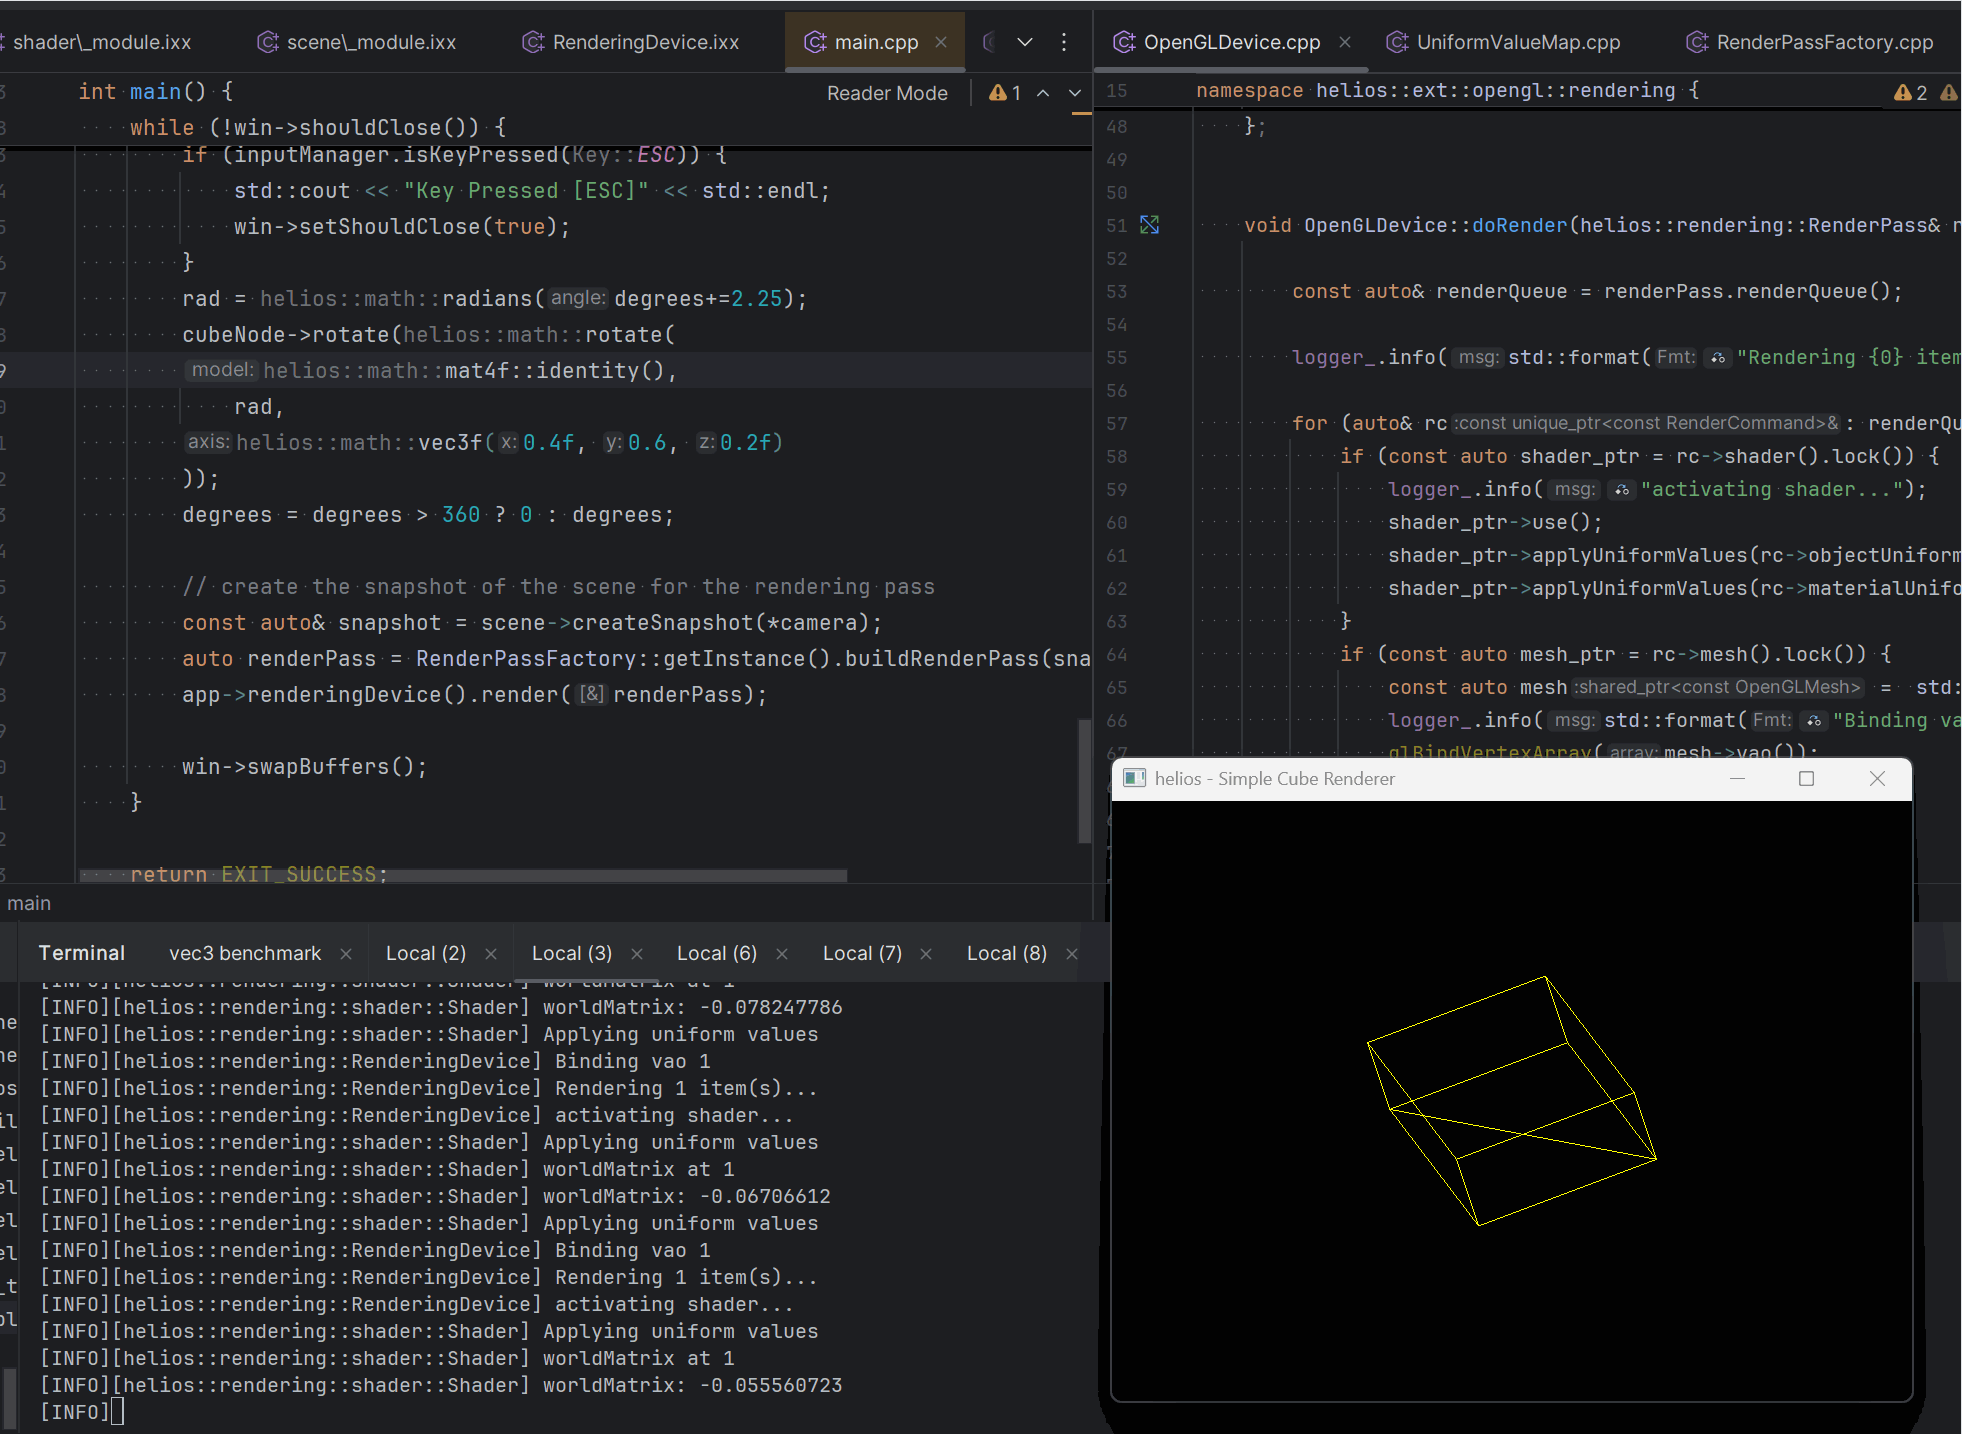
\includegraphics[width=1\columnwidth]{img/cube_example}
    \caption{Screenshot des \texttt{simple\_cube\_rendering}-demos, der zur Fertigstellung des ersten Meilensteins genutzt wurde.}
    \label{fig:simple-cube-rendering-demo}
\end{figure}

\subsection*{\texttt{/include, /src}}
Mit C++23 nutzt helios durchweg Module Interface und Implementation Units~\cite[211 f.]{Str24}, die in \texttt{/include} bzw. \texttt{/src} abgelegt werden.\par
Module, die nicht in interface und implementation units aufgeteilt werden, liegen ausschließlich in \texttt{/include} als ``header-only``-Komponenten.
Hierzu gehören Klassen wie \texttt{helios::math::vec3}, die einen dreidimensionalen Vektor-Typ repräsentieren und deren Funktionen überwiegend als \texttt{constexpr} deklariert sind\footnote{
    \texttt{constexpr} erlaubt die Evaluierung eines Ausdrucks zur Kompilierzeit. Hierzu wird dessen vollständige Definition zur Übersetzungszeit benötigt~\cite[330 f.]{Gre24}.
}.\par
Die Verzeichnisse sind weiter unterteilt in \textt{ext} und \texttt{helios}:
\begin{itemize}
    \itemsep0.5em
    \item \texttt{ext} beinhaltet plattformspezifische Implementierungen von Schnittstellen, die vom helios Framework vertraglich vorgegeben werden (hardwarenahe Window-/Applikations-Abstraktionen, außerdem Spezifika der Rendering-Pipeline).
    \item \texttt{helios} beinhaltet den eigentlichen Framework-Code
\end{itemize}